\documentclass[aspectratio=169]{beamer}
\usepackage[english]{babel}
\usepackage[UTF8,noindent]{ctex}
\usepackage{graphicx}
\usepackage{listings}
\usepackage{lmodern}  % for bold teletype font
\usepackage{amsmath}  % for \hookrightarrow
\usepackage{xcolor}

\lstset{
  basicstyle=\ttfamily,
  % columns=fullflexible,
  % frame=single,
  numbers=left,
  breaklines=true,
  % postbreak=\mbox{\textcolor{red}{$\hookrightarrow$}\space},
}

% 加导航条
\useoutertheme[width=3\baselineskip,right]{sidebar}
% 目录标数字
\setbeamertemplate{section in toc}[sections numbered] 
% 无序列表用实心点
\setbeamertemplate{itemize item}{$\bullet$}
% 设置每页标题格式
\setbeamertemplate{frametitle}
  {\vspace{-0.5cm}
   \insertframetitle
   \vspace{-0.5cm}}
% 去掉下面没用的导航条
\setbeamertemplate{navigation symbols}{}
% 设置页脚格式
\makeatother
\setbeamertemplate{footline}
{
  \leavevmode%
  \hbox{%
  \begin{beamercolorbox}[wd=.4\paperwidth,ht=2.25ex,dp=1ex,center]{author in head/foot}%
    \usebeamerfont{author in head/foot}\insertshortauthor
  \end{beamercolorbox}

  \begin{beamercolorbox}[wd=.6\paperwidth,ht=2.25ex,dp=1ex,center]{title in head/foot}%
    \usebeamerfont{title in head/foot}\insertshorttitle\hspace*{13em}
    \insertframenumber{} / \inserttotalframenumber\hspace*{0ex}
  \end{beamercolorbox}}

  \vskip0pt%
}
\makeatletter


% 定义颜色
%\definecolor{alizarin}{rgb}{0.82, 0.1, 0.26} % 红色
%\definecolor{DarkFern}{HTML}{407428} % 绿色
%\colorlet{main}{DarkFern!100!white} % 第一种设置方法
%\colorlet{main}{red!70!black} % 第二种设置方法
\definecolor{bistre}{rgb}{0.24, 0.17, 0.12} % 黑色
\definecolor{mygrey}{rgb}{0.52, 0.52, 0.51} % 灰色
\colorlet{main}{green!50!black}
\colorlet{text}{bistre!100!white}

% 不同元素指定不同颜色, fg是本身颜色, bg是背景颜色, !num!改变数值提供渐变色
\setbeamercolor{title}{fg=main}
\setbeamercolor{frametitle}{fg=main}
\setbeamercolor{section in toc}{fg=text}
\setbeamercolor{normal text}{fg=text}
\setbeamercolor{block title}{fg=main,bg=mygrey!14!white}
\setbeamercolor{block body}{fg=black,bg=mygrey!10!white}
\setbeamercolor{qed symbol}{fg=main} % 证明结束后的框颜色
\setbeamercolor{math text}{fg=black}
% 设置页脚对应位置颜色
\setbeamercolor{author in head/foot}{fg=black, bg=mygrey!5!white}
\setbeamercolor{title in head/foot}{fg=black, bg=mygrey!5!white}
\setbeamercolor{structure}{fg=main, bg=mygrey!10!white} % 设置sidebar颜色

% 左右页间距的排版
\def\swidth{2.3cm}
\setbeamersize{sidebar width right=\swidth}
\setbeamersize{sidebar width left=\swidth}
\setbeamerfont{title in sidebar}{size=\scriptsize}
\setbeamerfont{section in sidebar}{size=\tiny}


%-------------------正文-------------------------%

\author{Wang Zhengru}
\title{OS Assignment 1: \\Compile and Boot a Linux Kernel}
\date{Oct 14, 2020}

\begin{document}

\frame[plain]{\titlepage}

\begin{frame}
  \frametitle{Outline}
  \tableofcontents
\end{frame}

\section{System Info}

\begin{frame}{Outline}
  \tableofcontents[currentsection]
\end{frame}

\begin{frame}
  \frametitle{System Info}
  \begin{itemize}
    \item OS : ESXi-6.7.0-8169922-standard-customized (VMware, Inc.)
    \item CPU : Intel(R) Xeon(R) CPU E5-2620 @ 2.00GHz * 2
    \item VMOS : Ubuntu 20.04.1 LTS
    \item vCPU : 12 Cores, 24 Threads
    \item vRAM : 4 GiB
    % \item Storage : 200 GiB
  \end{itemize}
  \vspace{0.4cm}
  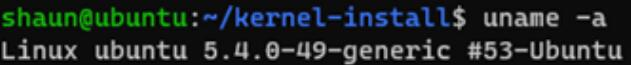
\includegraphics[width=9cm]{uname-old.jpg}
\end{frame}

\section{Compile}

\begin{frame}{Compile}
  \tableofcontents[currentsection]
\end{frame}

\subsection{Download}

\begin{frame}
  \frametitle{Download}
  \centering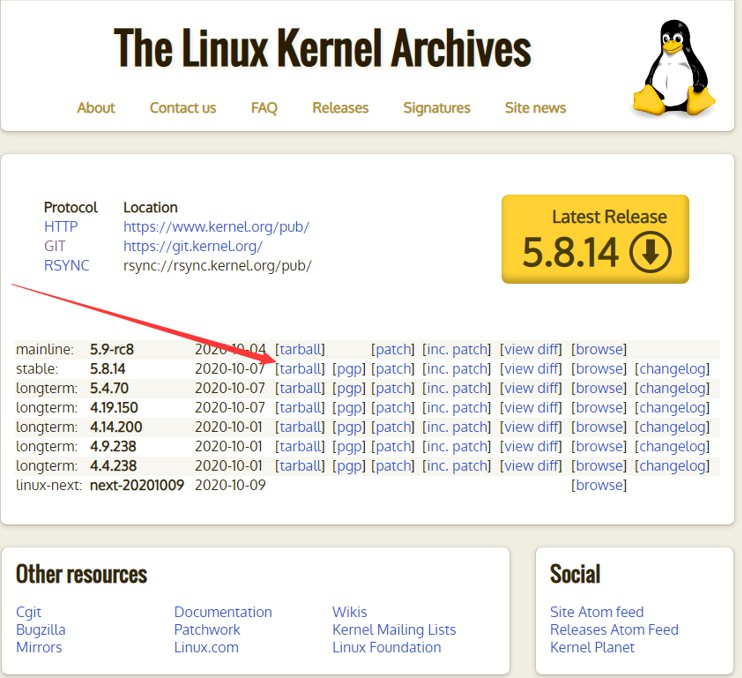
\includegraphics[width=6cm]{kernel-org.jpg}
  % wget https://cdn.kernel.org/pub/linux/kernel/v5.x/linux-5.8.14.tar.xz
  % \lstinputlisting[]{1.cpp}
\end{frame}

\begin{frame}
  \frametitle{Download}
  \centering
\includegraphics[width=10.5cm]{github-kernel.jpg}
  % wget https://cdn.kernel.org/pub/linux/kernel/v5.x/linux-5.8.14.tar.xz
  % \lstinputlisting[]{1.cpp}
\end{frame}

\begin{frame}
  \frametitle{Download}
  % \centering
\includegraphics[width=10.5cm]{github-kernel.jpg}
  % wget https://cdn.kernel.org/pub/linux/kernel/v5.x/linux-5.8.14.tar.xz
  \lstinputlisting[language=bash]{download.sh}
\end{frame}

\subsection{Compile}

\begin{frame}
  \frametitle{Config}
  \centering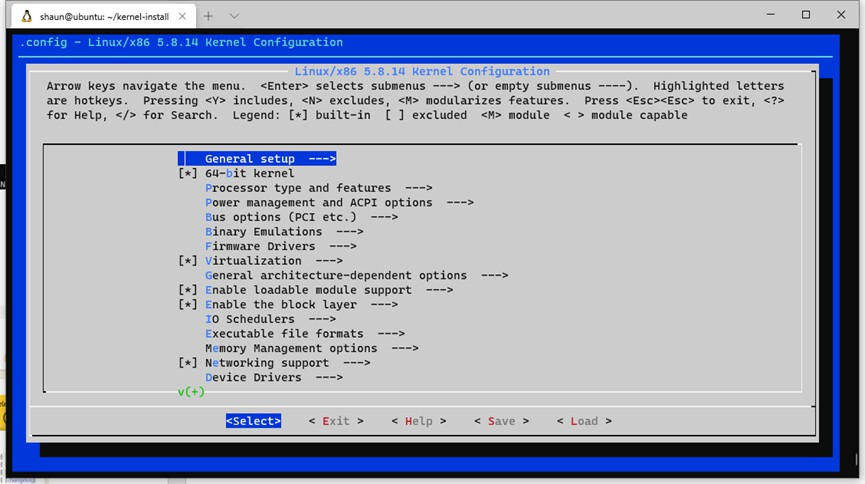
\includegraphics[width=10.5cm]{menuconfig.jpg}
  % wget https://cdn.kernel.org/pub/linux/kernel/v5.x/linux-5.8.14.tar.xz
  % \lstinputlisting[]{1.cpp}
\end{frame}

\begin{frame}
  \frametitle{Compile}
  \lstinputlisting[language=bash]{compile.sh}
\end{frame}

\begin{frame}
  \frametitle{A few moments later...}
  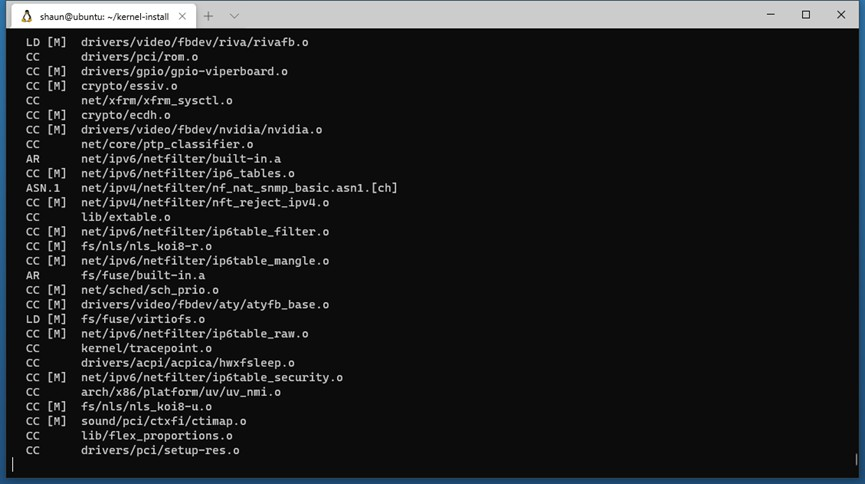
\includegraphics[width=9cm]{make.jpg}
  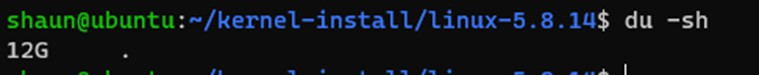
\includegraphics[width=9cm]{du-sh.jpg}
\end{frame}

\subsection{Install}

\begin{frame}
  \frametitle{Install}
  \lstinputlisting[language=bash]{install.sh}
  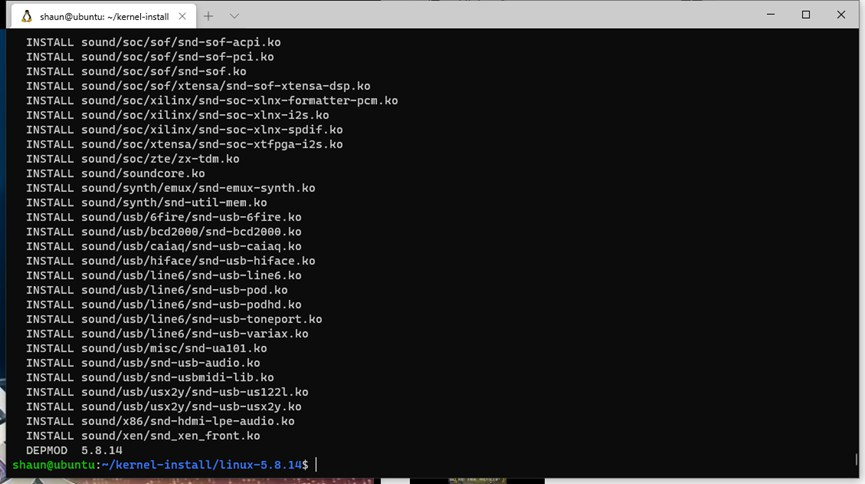
\includegraphics[width=9cm]{modules-install.jpg}
\end{frame}

\begin{frame}
  \frametitle{Bug!}
  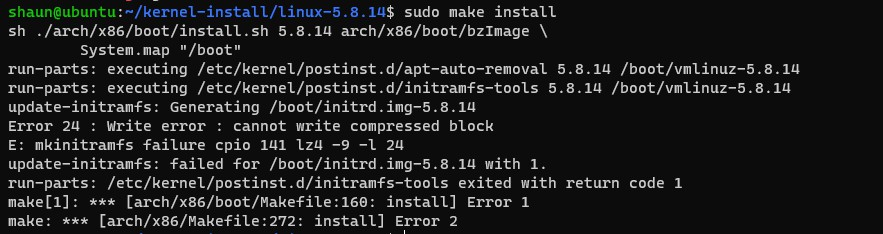
\includegraphics[width=10cm]{install-bug.jpg}
  \lstinputlisting[language=bash]{fix-install-bug.sh}
\end{frame}

\begin{frame}
  \frametitle{Install}
  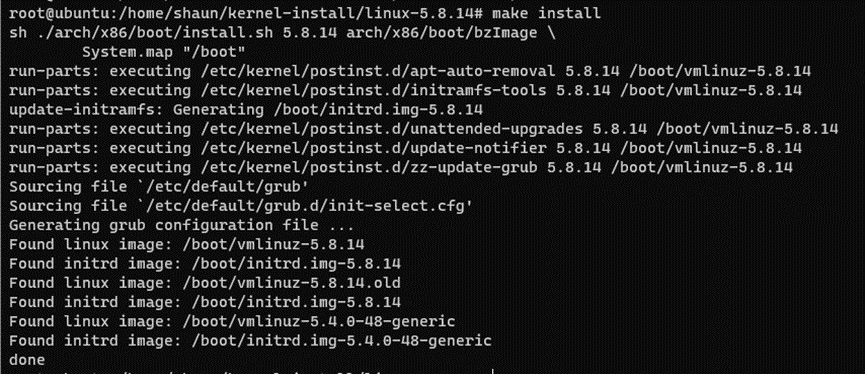
\includegraphics[width=9cm]{install.jpg}
\end{frame}

\section{Boot}

\subsection{Update GRUB}

\begin{frame}
  \frametitle{Update GRUB}
  sudo update-grub\\
  \vspace{2cm}
  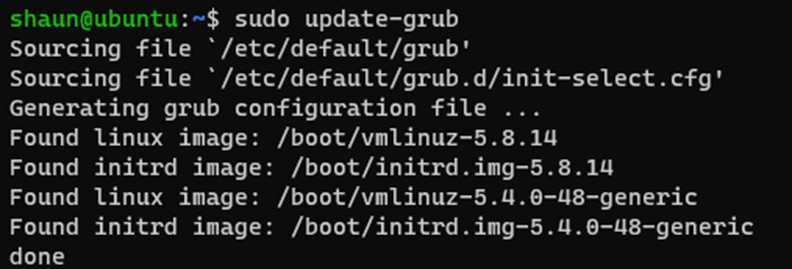
\includegraphics[width=9cm]{update-grub.jpg}
\end{frame}

\subsection{Reboot}

\begin{frame}
  \frametitle{Reboot and Enjoy}
  reboot\\
  uname -r\\
  \vspace{2cm}
  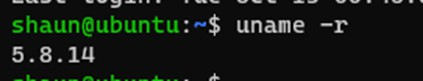
\includegraphics[width=9cm]{uname-new.jpg}
\end{frame}

\begin{frame}
  \frametitle{END}
  Thanks.
\end{frame}

\end{document}